\chapter{Tag 11 — Datamatrix: Anatomie und ASCII-Encoding}

\begin{quote}
Heute beginnt das große Finale: wir bauen einen Datamatrix-Code von
Grund auf. Datamatrix ist 2D, hat eingebaute Fehlerkorrektur (Reed-
Solomon — den Stoff aus Tag 6 bis 8) und ist auf Versandetiketten,
Werkstücken und in Krankenhäusern allgegenwärtig. Die nächsten vier
Etappen bauen das Symbol Schritt für Schritt: heute die Anatomie und
die erste Übersetzungsstufe (Text → Bytes), in den folgenden Tagen
die Reed-Solomon-Prüfsymbole, das berühmte „Treppenmuster" der
Datenplatzierung, und am Ende ein komplettes, von Hand gezeichnetes
Symbol.
\end{quote}

\section*{Lernziele für heute}

Am Ende von Tag 11 kannst du \dots

\begin{itemize}
\item die Bauteile eines Datamatrix-Symbols benennen (L-Pattern,
  Zeitsignal, Datenbereich)
\item die wichtigsten Symbol-Größen aus dem Datamatrix-Standard
  unterscheiden und sagen, wie viele Daten- und Prüfbytes in welcher
  Größe stecken
\item ein Wort wie \texttt{HONIG} im ASCII-Modus von Hand in
  Codewort-Bytes übersetzen
\item das gleiche in Python machen — und verstehen, warum bei
  Datamatrix \texttt{ord(ch) + 1} statt \texttt{ord(ch)} steht
\end{itemize}

\paragraph{Material} Bleistift, Karopapier, ASCII-Tabelle (steht
gleich am Anfang von Block 11.3), Laptop mit Thonny und Pillow.

% =============================================================
\section{Anatomie eines Datamatrix \normalfont(\textit{≈ 25 min})}
% =============================================================

So sieht ein fertiges Datamatrix-Symbol aus, das das Wort
\texttt{HONIG} kodiert (echtes, scannbares Symbol — 12 Module breit
und 12 hoch):

\begin{center}
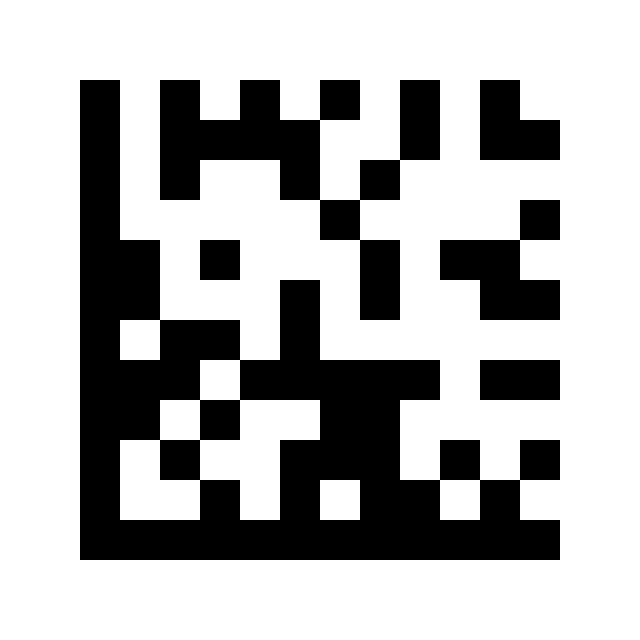
\includegraphics[width=4cm]{abbildungen/tag11/honig_dm_zoom.png}
\end{center}

Schwarze und weiße Quadrate (\textbf{Module}) in einem festen Raster.
Jedes Modul ist gleich groß; die Anzahl der Module pro Seite ist
genormt (10, 12, 14, 16, \dots~bis 144). Ein Datamatrix hat keine
„oben/unten" oder „links/rechts" — der Scanner findet die richtige
Orientierung am Rand.

\subsection*{Die drei Bauteile}

Jedes Datamatrix-Symbol setzt sich aus drei Teilen zusammen:

\begin{itemize}
\item \textbf{L-Pattern} (auch „Finder Pattern"). Zwei zusammenhängende
  schwarze Kanten, die den Buchstaben „L" bilden — am unteren und
  linken Rand des Symbols. Daran erkennt der Scanner die Orientierung.
\item \textbf{Zeitsignal} (auch „Timing Pattern"). Zwei abwechselnde
  schwarz-weiß-Kanten am oberen und rechten Rand, gegenüber dem
  L-Pattern. Daran erkennt der Scanner die Modul-Breite.
\item \textbf{Datenbereich}. Das Innere — hier stecken die eigentlichen
  Daten plus die Reed-Solomon-Prüfbytes. Schwarz-weiß-Module nach
  einem festen Algorithmus angeordnet (das berühmte „Treppenmuster",
  Stoff von Etappe 13).
\end{itemize}

L-Pattern und Zeitsignal sind \emph{immer gleich} — bei jedem
Datamatrix-Symbol derselben Größe. Nur die Module im Datenbereich
ändern sich je nach Inhalt.

\begin{bleistiftuebung}{1}{Bauteile am Symbol erkennen}
Schau dir den \texttt{HONIG}-Datamatrix oben an. Welche Kanten
gehören zum L-Pattern (also den festen schwarzen Rändern)? Welche
zum Zeitsignal (den abwechselnden Kanten)? Wo liegt der Datenbereich?

(Tipp: das L liegt unten links, mit der senkrechten Linie nach oben
und der waagrechten nach rechts — ähnlich wie ein Sitzplatz-„L".
Das Zeitsignal ist gegenüber.)
\end{bleistiftuebung}

\subsection*{Warum das Ganze?}

Vergleich mit EAN-13: dort steckte die ganze Information in einer
Zeile mit fester Breite (95 Module). Datamatrix nutzt die Fläche aus
— bei einem 12$\times$12-Symbol sind das $12 \cdot 12 = 144$ Module,
abzüglich Rand $\approx$ 96 Datenmodule. Das reicht für 12 Codewörter à
8 Bits. Bei 16$\times$16 sind es $144 + 12 \cdot 8 = 240$ Module für
24 Codewörter — entsprechend mehr Inhalt.

Und der wichtige Unterschied: bei jeder Symbol-Größe sind \emph{einige
der Codewörter Reed-Solomon-Prüfbytes}. Datamatrix kann beschädigte
Module rekonstruieren — etwas, was EAN-13 nicht kann.

% =============================================================
\section{Symbol-Größen und Codewort-Kapazitäten \normalfont(\textit{≈ 10 min})}
% =============================================================

Datamatrix kennt eine ganze Familie von Symbol-Größen. Jede Größe hat
eine festgelegte Aufteilung in Daten- und Prüfbytes. Für unsere
Test-Wörter HONIG, GRETA (je 5 Buchstaben) brauchen wir mindestens 5
Datenbytes — das ist das 12$\times$12-Symbol:

\begin{center}
\small
\begin{tabular}{c c c c}
\toprule
\textbf{Symbol} & \textbf{Module gesamt} & \textbf{Datenbytes} & \textbf{Prüfbytes (ECC)} \\
\midrule
10$\times$10  & 100  & 3   & 5   \\
\textbf{12$\times$12}  & \textbf{144}  & \textbf{5}   & \textbf{7}   \\
14$\times$14  & 196  & 8   & 10  \\
16$\times$16  & 256  & 12  & 12  \\
18$\times$18  & 324  & 18  & 14  \\
20$\times$20  & 400  & 22  & 18  \\
\dots         &      &     &     \\
\bottomrule
\end{tabular}
\end{center}

In den nächsten Etappen arbeiten wir mit \textbf{12$\times$12}: 5
Datenbytes für unsere fünf Buchstaben, 7 Prüfbytes für die
Fehlerkorrektur — total 12 Codewörter (mal 8 Bits = 96 Bits =
96 Datenmodule, plus L-Pattern und Zeitsignal: 144 Module = 12$\times$12).

Bemerkenswert: bei Datamatrix wachsen die Prüfbytes nicht linear mit
der Symbol-Größe — bei 12$\times$12 sind 7 von 12 Codewörtern Prüfbytes
(58 \% der Kapazität!), bei 16$\times$16 nur noch 12 von 24 (50 \%),
bei 144$\times$144 sind es nur noch 30 \%. Kleine Symbole sind also
besonders robust.

% =============================================================
\section{ASCII-Encoding: vom Buchstaben zum Codewort \normalfont(\textit{≈ 30 min})}
% =============================================================

Bevor die Reed-Solomon-Mathematik losgeht (Etappe 12), müssen wir
den Klartext in Codewort-Bytes übersetzen. Datamatrix kennt mehrere
Encoding-Modi (ASCII, C40, Text, Base 256, X12, EDIFACT) — wir nehmen
den einfachsten und universellsten: \textbf{ASCII-Modus}.

\subsection*{ASCII zur Erinnerung}

Jedes druckbare Zeichen hat im ASCII-Standard eine Nummer zwischen 32
und 126:

\begin{center}
\small\ttfamily
\begin{tabular}{c|c|c|c|c|c|c|c|c|c|c|c|c}
\toprule
A & B & C & D & E & F & G & H & I & J & \dots & Y & Z \\
65 & 66 & 67 & 68 & 69 & 70 & 71 & 72 & 73 & 74 & \dots & 89 & 90 \\
\bottomrule
\end{tabular}
\end{center}

In Python liefert die eingebaute Funktion \texttt{ord('H')} den Wert
\texttt{72} zurück. \texttt{chr(72)} geht den umgekehrten Weg.

\subsection*{Datamatrix-Offset: warum +1?}

Der Datamatrix-Standard reserviert die Bytes 0 (Padding-Pseudo-Random),
1--128 (ASCII-Codewörter), 129 (Pad-Byte), 130--229 (Doppelziffern)
und einige Steuer-Werte für andere Modi. ASCII-Codewort \texttt{n}
entspricht dem Zeichen mit ASCII-Wert \texttt{n - 1}. Anders gesagt:

\begin{quote}
\textbf{ASCII-Wert + 1 = Datamatrix-Codewort-Byte}
\end{quote}

Daher ist der Codewort-Wert für \texttt{'H'} nicht 72, sondern
\textbf{73}. Für \texttt{'A'} ist es \textbf{66}, für \texttt{'Z'} ist
es \textbf{91}.

\begin{bleistiftuebung}{2}{HONIG zu Codewort-Bytes}
Übersetze das Wort \texttt{HONIG} von Hand in eine Folge von
Codewort-Bytes nach der Datamatrix-ASCII-Regel. Schreibe dazu eine
kleine Tabelle:

\begin{center}
\small
\begin{tabular}{c c c}
\toprule
Buchstabe & ASCII-Wert (\texttt{ord}) & Codewort (\texttt{ord+1}) \\
\midrule
H & 72 & 73 \\
O & ?  & ?  \\
N & ?  & ?  \\
I & ?  & ?  \\
G & ?  & ?  \\
\bottomrule
\end{tabular}
\end{center}

(Die ASCII-Werte: \texttt{O}=79, \texttt{N}=78, \texttt{I}=73,
\texttt{G}=71.)
\end{bleistiftuebung}

\subsection*{Datamatrix-ASCII in Python}

Drei Mini-Funktionen — der Trick steht alles in einer Zeile pro
Funktion:

\begin{pythoneinheit}{1}{ASCII-Offset für ein Zeichen}
\pythoncodeteil{tag11/ascii_encoding.py}{offset}

\texttt{ord(ch)} liefert den ASCII-Wert, plus eins. Probier es in
der Thonny-Konsole für andere Buchstaben.
\end{pythoneinheit}

\begin{pythoneinheit}{2}{Ein ganzes Wort übersetzen}
\pythoncodeteil{tag11/ascii_encoding.py}{wort}

Eine Liste von Codewort-Bytes für ein ganzes Wort. Diese Schreibweise
\texttt{[buchstabe\_zu\_byte(ch) for ch in text]} heißt
\textbf{List Comprehension} — kompakte Form für „bau eine Liste, in
der für jedes \texttt{ch} aus \texttt{text} der Wert
\texttt{buchstabe\_zu\_byte(ch)} steht". Du hast das gleiche Muster
schon implizit in Tag 1 gesehen, aber explizit zum ersten Mal hier.
\end{pythoneinheit}

\subsection*{Padding: was, wenn das Wort zu kurz ist?}

Unser \texttt{HONIG} hat genau 5 Buchstaben — passt exakt in die 5
Datenbytes eines 12$\times$12-Symbols. Aber was, wenn wir nur 3
Buchstaben kodieren (z. B. \texttt{HON})? Dann müssen wir die
restlichen Datenbytes auffüllen — Datamatrix nennt das
\textbf{Padding} und nutzt dafür den festen Wert \texttt{129}.

\begin{pythoneinheit}{3}{Padding}
\pythoncodeteil{tag11/ascii_encoding.py}{padding}

Bei 5 Datenbytes Kapazität und 5 Buchstaben passt es genau, kein
Padding nötig. Bei kürzeren Wörtern stehen am Ende
\texttt{129}-Bytes, die der Decoder als „nichts mehr drin" erkennt.

(Datamatrix verwendet ab dem zweiten Pad-Byte tatsächlich eine
Pseudo-Random-Folge statt 129 — das macht das Symbol visuell
„zufälliger" und damit fehlertoleranter. Wir sparen uns das Detail
für den Polish-Sprint, der einfache Pad-Wert reicht für unsere
12$\times$12-Symbole mit voller Datenkapazität.)
\end{pythoneinheit}

\begin{bleistiftuebung}{3}{Greta vorbereiten}
Wähle ein eigenes 5-Buchstaben-Wort (z. B. \texttt{GRETA}) und
schreibe die Codewort-Byte-Folge dafür auf. Du wirst diese Folge
in Etappe 12 brauchen — dann berechnen wir die zugehörigen
Reed-Solomon-Prüfbytes.

(Tipp: \texttt{G}=71, \texttt{R}=82, \texttt{E}=69, \texttt{T}=84,
\texttt{A}=65 in ASCII.)
\end{bleistiftuebung}

% =============================================================
\section{Reflexion und Brücke zu Tag 12 \normalfont(\textit{≈ 5 min})}
% =============================================================

Du hast jetzt:

\begin{itemize}
\item ein Bild im Kopf, wie ein Datamatrix-Symbol aussieht und welche
  Bauteile es hat
\item gewusst, dass für 5 Buchstaben das 12$\times$12-Symbol passt
  (5 Datenbytes + 7 Prüfbytes = 12 Codewörter)
\item das ASCII-Encoding mit dem Datamatrix-Offset verstanden — sowohl
  von Hand als auch in Python
\end{itemize}

Was noch fehlt, bevor wir das Symbol zeichnen können:

\begin{itemize}
\item die \textbf{Reed-Solomon-Prüfbytes} berechnen (Tag 12) — und
  zwar mit dem Encoder, den wir in Tag 7 selbst gebaut haben.
\item die 12 Codewörter im Modul-Raster nach dem
  \textbf{Datenplatzierungs-Algorithmus} (Tag 13) verteilen.
\item L-Pattern und Zeitsignal drumherum, scannen, fertig (Tag 14).
\end{itemize}

\subsection*{Vorschau Tag 12}

Du nimmst dein \texttt{HONIG}-Codewort \texttt{[73, 80, 79, 74, 72]}
und gehst damit zum Reed-Solomon-Encoder aus Tag 7 (der mit
GF($2^8$) und Generator-Polynom $g(x)$). Heraus kommt eine 7-Byte-
Prüffolge — und plötzlich macht „klick", warum wir uns die
Polynomdivision in einem endlichen Körper überhaupt angetan haben.
